\documentclass{beamer}

% Beamer style
%\usetheme[secheader]{Madrid}
\usetheme{CambridgeUS}
\usecolortheme[rgb={0.65,0.15,0.25}]{structure}
%\usefonttheme[onlymath]{serif}
\beamertemplatenavigationsymbolsempty
%\AtBeginSubsection

% Packages
%\usepackage[french]{babel}
\usepackage[latin1]{inputenc}
\usepackage{color}
%\usepackage{dsfont, stmaryrd}
\usepackage{amsmath, amsfonts, amssymb}
\usepackage{epsfig}
\usepackage{url}
\usepackage{/media/donnees/LATEX/astats}
%\usepackage[all]{xy}
\usepackage{graphicx}

% Commands
\definecolor{darkred}{rgb}{0.65,0.15,0.25}
\newcommand{\emphase}[1]{\textcolor{darkred}{#1}}
%\newcommand{\emphase}[1]{{#1}}
\newcommand{\paragraph}[1]{\textcolor{darkred}{#1}}
\newcommand{\refer}[1]{[{\footnotesize{\textcolor{blue}{{\cite{#1}}}}}]}
\newcommand{\Refer}[1]{[{\footnotesize{\textcolor{blue}{{\sl #1}}}}]}
\newcommand{\newblock}{}

% Symbols
\newcommand{\Abf}{{\bf A}}
\newcommand{\Beta}{\text{B}}
\newcommand{\Bcal}{\mathcal{B}}
\newcommand{\BIC}{\text{BIC}}
\newcommand{\Ccal}{\mathcal{C}}
\newcommand{\dd}{\text{~d}}
\newcommand{\dbf}{{\bf d}}
\newcommand{\Dcal}{\mathcal{D}}
\newcommand{\Esp}{\mathbb{E}}
\newcommand{\Ebf}{{\bf E}}
\newcommand{\Ecal}{\mathcal{E}}
\newcommand{\Gcal}{\mathcal{G}}
\newcommand{\Gam}{\mathcal{G}\text{am}}
\newcommand{\Ibb}{\mathbb{I}}
\newcommand{\Ibf}{{\bf I}}
\newcommand{\ICL}{\text{ICL}}
\newcommand{\Cov}{\mathbb{C}\text{ov}}
\newcommand{\Corr}{\mathbb{C}\text{orr}}
\newcommand{\Var}{\mathbb{V}}
\newcommand{\Vsf}{\mathsf{V}}
\newcommand{\pen}{\text{pen}}
\newcommand{\Fcal}{\mathcal{F}}
\newcommand{\Hbf}{{\bf H}}
\newcommand{\Hcal}{\mathcal{H}}
\newcommand{\Jcal}{\mathcal{J}}
\newcommand{\Kbf}{{\bf K}}
\newcommand{\Lcal}{\mathcal{L}}
\newcommand{\Mcal}{\mathcal{M}}
\newcommand{\mbf}{{\bf m}}
\newcommand{\mum}{\mu(\mbf)}
\newcommand{\Ncal}{\mathcal{N}}
\newcommand{\Nbf}{{\bf N}}
\newcommand{\Nm}{N(\mbf)}
\newcommand{\Ocal}{\mathcal{O}}
\newcommand{\Obf}{{\bf 0}}
\newcommand{\Omegas}{\underset{s}{\Omega}}
\newcommand{\Pbf}{{\bf P}}
\newcommand{\Pcal}{\mathcal{P}}
\newcommand{\Qcal}{\mathcal{Q}}
\newcommand{\Rbb}{\mathbb{R}}
\newcommand{\Rcal}{\mathcal{R}}
\newcommand{\sbf}{{\bf s}}
\newcommand{\Sbf}{{\bf S}}
\newcommand{\Scal}{\mathcal{S}}
\newcommand{\Ucal}{\mathcal{U}}
\newcommand{\Vcal}{\mathcal{V}}
\newcommand{\Tbf}{{\bf T}}
\newcommand{\ubf}{{\bf u}}
\newcommand{\Ubf}{{\bf U}}
\newcommand{\Wbf}{{\bf W}}
\newcommand{\xbf}{{\bf x}}
\newcommand{\Xbf}{{\bf X}}
\newcommand{\ybf}{{\bf y}}
\newcommand{\Ybf}{{\bf Y}}
\newcommand{\zbf}{{\bf z}}
\newcommand{\Zbf}{{\bf Z}}
\newcommand{\betabf}{\text{\mathversion{bold}{$\beta$}}}
\newcommand{\pibf}{\text{\mathversion{bold}{$\pi$}}}
\newcommand{\phibf}{\text{\mathversion{bold}{$\phi$}}}
\newcommand{\Sigmabf}{\text{\mathversion{bold}{$\Sigma$}}}
\newcommand{\gammabf}{\text{\mathversion{bold}{$\gamma$}}}
\newcommand{\mubf}{\text{\mathversion{bold}{$\mu$}}}
\newcommand{\nubf}{\text{\mathversion{bold}{$\nu$}}}
\newcommand{\Thetabf}{\text{\mathversion{bold}{$\Theta$}}}
\newcommand{\thetabf}{\text{\mathversion{bold}{$\theta$}}}
\newcommand{\BP}{\text{BP}}
\newcommand{\EM}{\text{EM}}
\newcommand{\VEM}{\text{VEM}}
\newcommand{\VBEM}{\text{VBEM}}
\newcommand{\cst}{\text{cst}}
\newcommand{\obs}{\text{obs}}
\newcommand{\ra}{\emphase{\mathversion{bold}{$\rightarrow$}~}}
\newcommand{\QZ}{Q_{\Zbf}}
\newcommand{\Qt}{Q_{\thetabf}}
%\newcommand{\transp}{\text{{\tiny $\top$}}}
\newcommand{\transp}{\text{{\tiny \mathversion{bold}{$\top$}}}}

% Directory
\newcommand{\figmixt}{/media/donnees/ENSEIGN/COURS/MELANGE}
\newcommand{\figbma}{/media/donnees/RECHERCHE/RUPTURES/MELANGE/Exemples/Grippe}
\newcommand{\fignet}{/media/donnees/RECHERCHE/RESEAUX/EXPOSES/FIGURES}
\newcommand{\figeco}{/media/donnees/RECHERCHE/ECOLOGIE/EXPOSES/FIGURES}
%\newcommand{\figmotif}{/media/donnees/RECHERCHE/RESEAUX/Motifs/FIGURES}


%--------------------------------------------------------------------
\title[Averaging mixture models]{Averaging mixture models: a variational approximation}    

\author[S. Robin]{S. Robin \\
~ \\
joint with J.-J. Daudin, S. Li-Thao-T�, M.-L. Martin, S. Volant}

\institute[AgroParisTech / INRA]{
  \bigskip
  \begin{tabular}{ccccc}
    
\epsfig{file=\fignet/LogoINRA-Couleur.ps,
      width=2.5cm} & 
    \hspace{.5cm} &
    
\epsfig{file=\fignet/logagroptechsolo.eps,
      width=3.75cm} & 
    \hspace{.5cm} &
    
\epsfig{file=\fignet/logo-ssb.eps,
      width=2.5cm} \\ 
  \end{tabular} \\
  \bigskip
  }

\date[WGMBC'12]{Working Group on Model-Based Clustering, \\
  July 2012, Guelph, Canada}
%--------------------------------------------------------------------

%--------------------------------------------------------------------
%--------------------------------------------------------------------
\begin{document}
%--------------------------------------------------------------------
%--------------------------------------------------------------------

%--------------------------------------------------------------------
\frame{\titlepage}

%%--------------------------------------------------------------------
%\frame{ \frametitle{Outline}
%  \tableofcontents}

%--------------------------------------------------------------------
%--------------------------------------------------------------------
\section{Introduction}
\frame{\frametitle{Introduction}}
%--------------------------------------------------------------------
  
%--------------------------------------------------------------------
\frame{\frametitle{Mixtures for density estimation}

  Mixture models
  $$
  g_K(x) = \sum_{k=1}^K \pi_k f(x; \gamma_k)
  $$
  \begin{itemize}
  \item are useful for model-based clustering
  \item but also provide \emphase{flexible density estimates} \\
    \ra intermediate between fully parametric and non-parametric (e.g. kernel) estimates.
  \end{itemize}

  \bigskip\bigskip \pause
  For density estimation, the number of groups $K$ has no real interest: 
  \begin{itemize}
  \item selecting the 'true' $K$ does not really make sense;
  \item combining the estimates via \emphase{model averaging} seems natural:
    $$
    \widehat{g}(x) = \sum_K w_K \widehat{g}_K(x).
    $$
  \end{itemize}
}

%--------------------------------------------------------------------
\frame{\frametitle{Binary classification problem}

  \begin{tabular}{cc}
    \hspace{-.5cm}
    \begin{tabular}{p{.5\textwidth}}
      \onslide+<1->{
        \paragraph{Aim = } 
        Determine epidemics periods vs normal behavior.
      }     

      \onslide+<2->{
        \bigskip
        \paragraph{Binary unsupervised classification}
        where one distribution is known:
        $$
        g(x) = \pi_0 \textcolor{red}{\phi(x)} + (1-\pi_0)
        \textcolor{blue}{f(x)}.
        $$
      }

      \onslide+<4->{
        The alternative distribution $f$ can be
        modeled as
        $$
        f(x) = \sum_{k=1}^K \pi_k h(x; \gamma_k)
        $$
      }
      
%      \onslide+<9->{
%        \bigskip
%        \paragraph{Model averaging.}
%        $$
%        \widehat{\tau} = \sum_K w_K \widehat{\tau}_K
%        $$
%      }

      \onslide+<9->{
        Similar to \emphase{local FDR} estimation.  
      }
    \end{tabular}
    &
    \hspace{-.5cm}
    \begin{tabular}{p{.45\textwidth}}
      \onslide+<1->{
        \paragraph{Influenza incidence rate:} Weekly data. \\
      }
      \begin{overprint}
        \onslide<1>
        \epsfig{file = \figbma/Grippe-NormHist.eps,             
          height=.5\textwidth, width=0.5\textheight,  clip=, angle=270} \\
        \onslide<2>
        \epsfig{file = \figbma/Grippe-NormHistH0.eps, 
          height=.5\textwidth, width=0.5\textheight,  clip=, angle=270} \\
        \onslide<3>
        \epsfig{file = \figbma/Grippe-Mixt-K1.eps,
          height=.5\textwidth, width=0.5\textheight, clip=, angle=270} \\   
        \onslide<4>
        \epsfig{file = \figbma/Grippe-Mixt-K2.eps,
          height=.5\textwidth, width=0.5\textheight, clip=, angle=270} \\   
        \onslide<5>
        \epsfig{file = \figbma/Grippe-Mixt-K3.eps, 
          height=.5\textwidth, width=0.5\textheight, clip=, angle=270} \\  
        \onslide<6>
        \epsfig{file = \figbma/Grippe-Mixt-K4.eps, 
          height=.5\textwidth, width=0.5\textheight, clip=, angle=270} \\  
        \onslide<7>
        \epsfig{file = \figbma/Grippe-Mixt-K5.eps, 
          height=.5\textwidth, width=0.5\textheight, clip=, angle=270} \\  
        \onslide<8->
        \epsfig{file = \figbma/Grippe-Mixt-K6.eps, 
          height=.5\textwidth, width=0.5\textheight, clip=, angle=270} \\  
%        \onslide<9->
%        \epsfig{file = \figbma/Grippe-Mixt-BMA.eps, 
%          height=.5\textwidth, width=0.5\textheight,  clip=, angle=270} 
      \end{overprint}
      \onslide+<1->{\refer{SuC09}} \\
      ~ \\
      ~ \\
      ~
    \end{tabular}
  \end{tabular}  

}

%--------------------------------------------------------------------
\frame{\frametitle{Species abundance estimation}

  \begin{tabular}{cc}
    \hspace{-.5cm}
    \begin{tabular}{p{.45\textwidth}}
      \onslide+<2->{
        \paragraph{Question:} 
        How many species are present, but unobserved? 
      }     
      
      \onslide+<3->{
        \bigskip
        \paragraph{Classical strategy:} 
        \begin{itemize}
        \item Fit the truncated distribution $g^+$; 
        \item Infer the proportion of $g(0)$ unobserved species.
        \end{itemize}
      }     
      
      \onslide+<4->{
        \bigskip
        \paragraph{'Non-parametric' approach:} \\
        Fit $g^+$ with a mixture $g_K^+$. \\
        ~
      }     
      
    \end{tabular}
    & 
    \hspace{-.5cm}
    \begin{tabular}{p{.5\textwidth}}
      \onslide+<1->{
        \paragraph{Data = } 
        Number of species observed $x$ times in a given area 
        \refer{FCW43} \\ }
      \begin{overprint}
        \onslide<1-2>
        \epsfig{file = \figeco/Butterfly.eps,
          height=.5\textwidth, width=0.5\textheight, clip=, angle=270} \\   
        \onslide<3>
        \epsfig{file = \figeco/Butterfly-MixtGeom-K1.eps,
          height=.5\textwidth, width=0.5\textheight, clip=, angle=270} \\   
        \onslide<4>
        \epsfig{file = \figeco/Butterfly-MixtGeom-K2.eps,
          height=.5\textwidth, width=0.5\textheight, clip=, angle=270} \\   
        \onslide<5>
        \epsfig{file = \figeco/Butterfly-MixtGeom-K4.eps, 
          height=.5\textwidth, width=0.5\textheight, clip=, angle=270} \\  
%        \onslide<6>
%        \epsfig{file = \figeco/Butterfly-MixtGeom-K4.eps, 
%          height=.5\textwidth, width=0.5\textheight, clip=, angle=270} \\  
      \end{overprint}
    \end{tabular}
  \end{tabular}

  \onslide+<4->{
    \paragraph{Estimated proportion of unobserved species:} 
    $
    \widehat{g}(0) = \sum_K w_K \widehat{g}_K(0).
    $
  }     
}

%--------------------------------------------------------------------
\section{Variational Bayes Model Averaging}
\frame{\frametitle{Variational Bayes Model Averaging (VBMA)}}
%--------------------------------------------------------------------

%--------------------------------------------------------------------
\frame{\frametitle{Bayesian model averaging (BMA)}

  \paragraph{Problem.} Consider a \emphase{parameter of interest
    $\delta = \delta(\thetabf)$} that can be estimated with different
  models $\Mcal_1, \Mcal_2, \dots, \Mcal_K, \dots$ \pause
  \begin{itemize}
  \item Classification: $\delta_t = \Pr\{t \in \text{epidemic} | \Xbf\}$
  \item Abundance: $\delta = g(0)$.
  \end{itemize}
  
  \bigskip\pause
  \paragraph{Bayesian model averaging.} 
  Average the estimates \refer{HMR99}:
  $$
  \emphase{\widehat{\delta}}  = \Esp(\delta|\Xbf) = \sum_K
  P(K|\Xbf) \Esp(\delta|\Xbf, K) =  \sum_K P(K|\Xbf)
  \emphase{\widehat{\delta}_K}.
  $$ \pause 
  or more generally
  $$
  P(\delta|\Xbf) = \sum_K P(K|\Xbf) P(\delta|\Xbf, K)
  $$

  \pause
  \paragraph{Question:} How to compute the weights
  $
  \emphase{w_K = P(K | \Xbf)}
  $?

 }

%--------------------------------------------------------------------
\frame{\frametitle{Variational Bayes (VB) inference}

  \paragraph{Variational Bayes inference} 
  aims at providing an approximation of the posterior distribution
  $$
  P(\thetabf | \Xbf).
  $$

  \bigskip\pause
  \paragraph{VB-EM.} 
  In presence of a hidden structure $\Zbf$, VB-EM \refer{BeG03}
  retrieves the \emphase{optimal approximation} of $P(\thetabf, \Zbf |
  \Xbf)$:
  $$ 
  Q(\Zbf, \thetabf) = \arg\min_{Q \in \Qcal} KL(Q(\theta, \Zbf); P(\thetabf, \Zbf
  | \Xbf))
  $$
  where $Q$ is factorisable:
  $
  \Qcal = \{Q: Q(\theta, \Zbf) = \Qt(\thetabf) \QZ(\Zbf)  \}
  $

  \bigskip\bigskip\pause
  \paragraph{Variational BMA.} 
  To combine models $\Mcal_1$, \dots, $\Mcal_K$, \dots, look for
  $$
  Q(\Zbf, \thetabf, \emphase{K}) \approx P(\Zbf, \thetabf, \emphase{K} | \Xbf)
  $$

}

%--------------------------------------------------------------------
\frame{\frametitle{Optimal weights}

  \paragraph{No additional approximation.} Consider the class
  $$
  \Qcal = \{Q: Q(\Zbf, \thetabf, \emphase{K}) = \QZ(\Zbf|K) \Qt(\thetabf|K)
  \emphase{Q_K(K)}\}
  $$ 
  we have $Q^*(\Zbf, \thetabf, K)$
  \begin{eqnarray*}
   & = & \emphase{\arg\min_{Q \in \Qcal}} KL[Q(\Zbf,
    \thetabf, K), P(\Zbf, \thetabf, K | \Xbf)] \pause \\ 
  & = & \emphase{\arg\min_{Q_K}} \left\{ 
    \begin{array}{ll}
      \displaystyle{KL(Q_K(K)), P(K|\Xbf))}  \\
      \\
      \displaystyle{+ \sum_K Q_K(K) \; \emphase{\arg\min_{\QZ, \Qt}} KL[Q(\Zbf,
    \thetabf| K), P(\Zbf, \thetabf | \Xbf, K)] } 
      \end{array}\right\}
  \end{eqnarray*}

  \bigskip\pause
  \paragraph{Optimal variation weights:} \refer{VMR12}
  \begin{eqnarray*}
    Q_K^*(K) & \propto & P(K) \exp \{\log P(\Xbf|K) - KL[Q^*(\Zbf,
    \thetabf|K); P(\Zbf,  \thetabf|\Xbf, K)]\} \\
    \\
    & = & \emphase{P(K|\Xbf)} e^
        {-{KL[Q^*(\Zbf, \thetabf|K); P(\Zbf, \thetabf|\Xbf,
            K)]}}.
  \end{eqnarray*}
  }

%--------------------------------------------------------------------
\frame{\frametitle{VBMA: the recipe}

  \paragraph{For $K = 1 \dots K_{\max}$} 
  \begin{itemize}
  \item Use regular VB-EM to compute the approximate conditional posterior 
    $$     
    Q^*_{\Zbf, \thetabf|K}(\Zbf, \thetabf|K) = Q^*_{\Zbf|K}(\Zbf|K)
    Q^*_{\thetabf|K}(\thetabf|K);
    $$ 
  \item Compute the conditional lower bound of the log-likelihood
    $$     
    \log P(\Xbf|K) - KL[Q^*(\Zbf, \thetabf|K); P(\Zbf,
      \thetabf|\Xbf, K)].    
    $$
  \end{itemize}

  \bigskip\pause
  \paragraph{Compute the approximate posterior of model $\Mcal_K$:} 
  $$
  w_K := Q_K(K) \propto P(K | \Xbf) \exp(-KL_K).
  $$ 

  \bigskip\pause
  \paragraph{Deduce the approximate posterior of $\delta$:} 
  $$
  P(\delta | \Xbf) \approx \sum_K w_K Q^*_{\thetabf | K}(\delta | K)
  $$
  }

%--------------------------------------------------------------------
\section{Applications}
\frame{\frametitle{Applications}}
%--------------------------------------------------------------------
\frame{\frametitle{Classification with HMM}

  \begin{tabular}{cc}
    \hspace{-.5cm}
    \begin{tabular}{p{.45\textwidth}}
      \onslide+<1->{
        \paragraph{Model.} 2-state (normal / epidemic) HMM
        \begin{eqnarray*}
          X_t & | & \text{epidemic} \sim f \\
          \delta_t & = & \Pr\{t \in \text{epidemic} | \Xbf\}
        \end{eqnarray*}
      }
      
      \onslide+<2->{
        \paragraph{$f = $ mixture:} Weights
        $$
        \begin{array}{ccccc}
          K & 2 & 3 & 4 & 5   \\
          \hline
          w_K & - & .34 & .66 & -
        \end{array}
        $$
      }
      
      \onslide+<3->{
        \paragraph{Classification}
        $$
        \widehat{\delta}(x_t) = \sum_K w_K \widehat{\delta}_K(x_t)
        $$
        $\widehat{\tau}_K$ for a $K$-component mixture.
      }
    \end{tabular}
    & 
    \hspace{-.5cm}
    \begin{tabular}{p{.5\textwidth}}
      \onslide+<1->{
        \paragraph{Influenza incidence rate:} Weekly data. \\
        \epsfig{file = ../Figures/VMR12-CSDA-Fig5.eps, 
          height=.58\textwidth, width=0.7\textheight, clip=,} \\
        }
    \end{tabular}
  \end{tabular}
}

%--------------------------------------------------------------------
\frame{\frametitle{Diversity of the human microbiome}
  
  \begin{tabular}{cc}
    \hspace{-.5cm}
    \begin{tabular}{p{.45\textwidth}}
       \paragraph{Mixture.} For $K = 1... K_{\max}$ we get
       $\widehat{g}_K(0)$ and 
       $$
       Q_K(g(0)) \approx 
       P(g(0) |K, \Xbf)
       $$

       \bigskip
       \paragraph{Model averaging.} 
       Estimate of the total number of present species \refer{LDR12}:  
       $$ 
       \emphase{\widehat{N} = 25,700}.
       $$
    \end{tabular}
    & 
    \hspace{-.5cm}
    \begin{tabular}{p{.5\textwidth}}
%       \epsfig{file = \figeco/LDR12-Fig1.eps, 
       \epsfig{file = \figeco/LDR10-42.eps, 
         height=.5\textheight, width=0.75\textwidth,  clip=}
    \end{tabular}
  \end{tabular}
  
  \pause
  \paragraph{Question:} 
  Can we provide a credibility interval for $g(0)$? 

  \medskip
  \paragraph{Problem:}   
  VB-E-M is prone to under-estimate the posterior variance
  \refer{McT09}.

}

%--------------------------------------------------------------------
\frame{\frametitle{Importance sampling}

  \begin{tabular}{cc}
    \hspace{-.5cm}
    \begin{tabular}{p{.45\textwidth}}
      \paragraph{Idea.} 
      Use $Q_K$ as a proposal: 
      \begin{eqnarray*}
      g^b(0) \text{ i.i.d.} & \sim & Q_K, \\
      \\
      \widehat{P}(g(0)|K) & \propto & \frac1B \sum_b \frac{P(g^b(0),
        \Xbf|K)}{Q_K(g^b(0))}.
      \end{eqnarray*}
%      $g^b(0)$ i.i.d. $\sim Q_K$, 
%      $$
%      \widehat{P}(g(0)|K) \propto \frac1B \sum_b \frac{P(g^b(0),
%        \Xbf|K)}{Q_K(g^b(0))}.
%      $$
      
      \bigskip
      \paragraph{Variational Bayes posterior} does not explore the
      whole range of the true posterior.  
    \end{tabular}
    & 
    %\hspace{-.5cm}
    \begin{tabular}{c}
      \pause
      \emphase{$\text{CI}_{95\%} = [19,421; 36,355]$} \\
      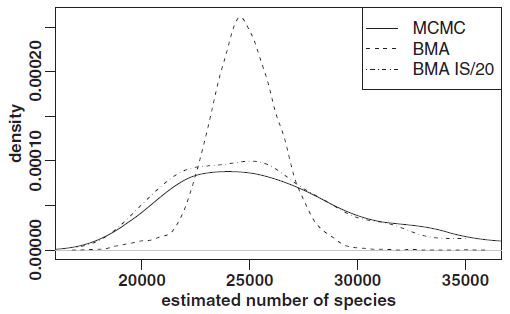
\epsfig{file = \figeco/LDR12-Fig6.eps, 
        height=.5\textheight, width=0.45\textwidth,  clip=} 
    \end{tabular}
  \end{tabular}

  \bigskip\pause
  \hspace{-0.25cm}
  \begin{tabular}{rrl}
    \paragraph{Variance inflation.} & Prior: & $\displaystyle{\Beta(a,
      b)}$ \\
    & Variational posterior: & $\displaystyle{\Beta(\widetilde{a},
      \widetilde{b})}$ \\
    & Inflated variational posterior: &
    $\displaystyle{\Beta\left({\widetilde{a}}/\emphase{v},
        {\widetilde{b}}/\emphase{v} \right)}$
  \end{tabular}
  }

%--------------------------------------------------------------------
\frame{\frametitle{Conclusion and future work}

  \paragraph{Variational Bayes model averaging}
  \begin{itemize}
  \item Allows to combine different model prediction,
  \item With the same complexity as regular (VB-)EM algorithms,
  \item With no additional approximation as for $p(\thetabf|\Xbf)$.
  \end{itemize}

  \pause\bigskip
  \paragraph{Variational Bayes model averaging (VBMA)}
  \begin{itemize}
  \item Seems to work well for classification ($\min KL$ preserves the
    mode \refer{Min05}),
  \item But needs to be combined with importance sampling to get
    reliable credibility intervals ($\min KL$ does not preserve the variance).
  \end{itemize}

  \pause\bigskip
  \paragraph{Future work.} Network modeling:
  \begin{itemize}
  \item $W$-graph = flexible network model based on a connectivity function 
    $$
    \phi: [0, 1] \times [0, 1] \rightarrow [0, 1]
    $$
  \item which can be approximated by averaging stochastic block-models.
  \end{itemize}
}

%--------------------------------------------------------------------
{\tiny
  \bibliography{/media/donnees/Biblio/ARC,/media/donnees/Biblio/AST,/media/donnees/Biblio/SSB}
  \bibliographystyle{/media/donnees/LATEX/astats}
  %\bibliographystyle{plain}
  }

%--------------------------------------------------------------------
\appendix
%-------------------------------------------------------------------- 
\section{Appendix}

%--------------------------------------------------------------------
%--------------------------------------------------------------------
\end{document}
%--------------------------------------------------------------------
%--------------------------------------------------------------------

  \begin{tabular}{cc}
    \hspace{-.5cm}
    \begin{tabular}{p{.5\textwidth}}
    \end{tabular}
    & 
    \hspace{-.5cm}
    \begin{tabular}{p{.5\textwidth}}
    \end{tabular}
  \end{tabular}
